\documentclass[12pt]{article}
\usepackage{polski}
\usepackage[utf8]{inputenc}
\usepackage[T1]{fontenc}
\usepackage{amsmath}
\usepackage{amsfonts}
\usepackage{fancyhdr}
\usepackage{lastpage}
\usepackage{multirow}
\usepackage{amssymb}
\usepackage{amsthm}
\usepackage{textcomp}
\frenchspacing
\usepackage{fullpage}
\setlength{\headsep}{30pt}
\setlength{\headheight}{12pt}
%\setlength{\voffset}{-30pt}
%\setlength{\textheight}{730pt}
\pagestyle{myheadings}
%\usepackage{kuvio,amscd,diagrams,dcpic,xymatrix,diagxy}
\usepackage{tikz,paralist,mathtools}
\usetikzlibrary{matrix,arrows,decorations}

\DeclareMathOperator{\coker}{coker}
\DeclareMathOperator{\Hom}{Hom}
\DeclareMathOperator{\Tor}{Tor}
\DeclareMathOperator{\Mor}{Mor}
\DeclareMathOperator{\Kom}{Kom}
\DeclareMathOperator{\sgn}{sgn}
\DeclareMathOperator{\Ext}{Ext}
\DeclareMathOperator{\Ob}{Ob}
\DeclareMathOperator{\Cone}{C}
\DeclareMathOperator{\Cyl}{Cyl}
\DeclareMathOperator{\Der}{D}
\DeclareMathOperator{\K}{K}
\newcommand{\Set}{\mathrm{Set}}
\newcommand{\Top}{\mathrm{Top}}
\newcommand{\Rmod}{\mathrm{R-mod}}
\newcommand{\id}{\mathrm{id}}
\newcommand{\A}{\mathcal{A}}
\newcommand{\B}{\mathcal{B}}
\newcommand{\C}{\mathcal{C}}
\newcommand{\D}{\mathcal{D}}
\newcommand{\Q}{\mathcal{Q}}
\newcommand{\qi}{quasi-isomorphism}

\newcommand{\bigslant}[2]{{\left.\raisebox{.2em}{$#1$}\middle/\raisebox{-.2em}{$#2$}\right.}}
\newcommand{\mf}[1]{{\mathfrak{#1}}}
\newcommand{\mb}[1]{{\mathbb{#1}}}
\newcommand{\mc}[1]{{\mathcal{#1}}}
\newcommand{\mr}[1]{{\mathrm{#1}}}


\newcounter{punkt}

\theoremstyle{plain}
\newtheorem{theorem}[punkt]{Theorem}
\newtheorem{lemma}[punkt]{Lemma}
\newtheorem{definition}[punkt]{Definition}
\newtheorem{fact}[punkt]{Fact}
\newtheorem{proposition}[punkt]{Proposition}
\newtheorem{corollary}[punkt]{Corollary}

\theoremstyle{definition}
\newtheorem{remark}[punkt]{Remark}
\newtheorem{example}[punkt]{Example}
\newtheorem{exercise}[punkt]{Exercise}



\markright{Piotr Suwara\hfill Homological algebra II: 1 September 2014\hfill}

\begin{document}

	We began with some motivation-discussion. 
	Ain't got time to write that nicely (in a~motivating way).
	
	\begin{theorem}[definition of derived category]
		Let $\C$ be an abelian category and $\Kom(\C)$ denote the category
		of cochain complexes over $\C$. 
		Then there is a~category $\Der(\C)$ (derived category of $\C$)
		and a~functor $\Q:\Kom(\C) \to \Der(\C)$
		such that
		\begin{enumerate}
			\item For every quasi-isomorphism $f \in \Mor(\Kom(\C))$,
			$\Q(f)$ is an isomorphism.
			
			\item $\Q$ is universal with respect to $1$, i.e.
			for every $\A$ and $F:\Kom(\C) \to \A$, such that
			for every \qi $f$ the map $F(f)$ is invertible,
			there exists $\Q F$ making the diagram commutative:
			
			\begin{tikzpicture}
				\matrix(m)[matrix of math nodes, row sep=1em]
				{\Kom(\C) & & \Der(\C) \\
				& \A & \\};
				\path[->,font=\scriptsize]
				(m-1-1) edge node[auto] {$\Q$} (m-1-3)
				(m-1-1) edge node[left] {$F$} (m-2-2)
				(m-1-3) edge node[right] {$\Q F$} (m-2-2);
			\end{tikzpicture}

		\end{enumerate}
		
		$\Der(\C)$ is called the \emph{derived category} of $\C$.
	\end{theorem}
	
	\begin{definition}[localisation of a~category]
		$\B$ is a~category, $S$ a~class of morphisms in $\B$.
		We can find a~new category $\B[S^{-1}]$ and a~functor
		$L:\B \to \B[S^{-1}]$ such that 
		for any functor $F: \B \to \B'$ which takes any $s \in S$
		to an isomorphism there exists a~functor $LF:\B[S^{-1}] \to \B'$
		such that
		
			\begin{tikzpicture}
				\matrix(m)[matrix of math nodes, row sep=1em]
				{\B & & \B[S^{-1}] \\
				& \B' & \\};
				\path[->,font=\scriptsize]
				(m-1-1) edge node[auto] {$L$} (m-1-3)
				(m-1-1) edge node[left] {$F$} (m-2-2)
				(m-1-3) edge node[right] {$: F$} (m-2-2);
			\end{tikzpicture}
	\end{definition}
	
	\begin{fact}
		$\Der(\C) = \Kom(\C)[(\mr{q-iso})^{-1}]$
	\end{fact}
	
	\begin{definition}
		The class $S \subset \Mor(\B)$ is localising if it satisfies
		\begin{itemize}
			\item $\forall_{X \in \Ob(\B)} \id_X \in S$
			\item $s, t \in S \implies s \circ t \in S$
			\item $\forall_{s \in S, f} \exists_{t \in S, g}$
			
			\begin{tikzpicture}
				\matrix(m)[matrix of math nodes, row sep=1em, column sep=1em]
				{ W & Z \\
				 X & Y \\};
				\path[->,font=\scriptsize]
				(m-1-1) edge node[auto] {$g$} (m-1-2)
				(m-1-1) edge node[auto] {$t$} (m-2-1)
				(m-2-1) edge node[auto] {$f$} (m-2-2)
				(m-1-2) edge node[auto] {$s$} (m-2-2);
			\end{tikzpicture}
			\item $\forall_{t \in S, g} \exists_{s \in S, f}$ as above
			\item $f,g : X \to Y$, then 
				$\exists_{s \in S} sf=sg \iff \exists_{t \in S} ft = gt$.
		\end{itemize}

	\end{definition}
	
	\begin{lemma}
		If $S$ is localizing in $\B$, then we can present any morphism in
		$\B[S^{-1}]$ as a~triangle $X \xleftarrow{s} Z \xrightarrow Y$
		with equivalence $(s,f) \sim (t,g) \iff \exists r \in S, h$
		
		\begin{tikzpicture}
			\matrix(m)[matrix of math nodes, row sep=1em, column sep=1em]
			{ & Z'' & \\
			Z & & Z' \\
			X & & Y \\};
			\path[dotted,->,font=\scriptsize]
			(m-1-2) edge node[auto] {$r$} (m-2-1)
				edge node[auto] {$h$} (m-2-3);
			\path[->,font=\scriptsize]
			(m-2-1) edge node[left] {$s$} (m-3-1)
				edge node[above left] {$f$} (m-3-3)
			(m-2-3) edge node[auto] {$g$} (m-3-3)
				edge node[above right] {$t$} (m-3-1);
		\end{tikzpicture}
		
		Also, an equivalent statement with left fractions is true.
	\end{lemma}
	
	\begin{lemma}[composition]Like that.
	
		\begin{tikzpicture}
			\matrix(m)[matrix of math nodes, row sep=1em, column sep=1em]
			{ & & X'' & & \\
			 & X' & & Y' & \\
			X & & Y & & Z \\};
			\path[dotted,->,font=\scriptsize]
			(m-1-3) edge node[auto] {$t'$} (m-2-2)
				edge node[auto] {$f'$} (m-2-4);
			\path[->,font=\scriptsize]
			(m-2-2) edge node[auto] {$s$} (m-3-1)
				edge node[auto] {$f$} (m-3-3)
			(m-2-4) edge node[auto] {$g$} (m-3-5)
				edge node[auto] {$t$} (m-3-3);
		\end{tikzpicture}
	\end{lemma}
	
	\begin{remark}
		Class of \qi is not localising in $\Kom(\C)$.
	\end{remark}




\end{document}
 
 
